% Created by tikzDevice version 0.12 on 2019-07-24 15:43:54
% !TEX encoding = UTF-8 Unicode
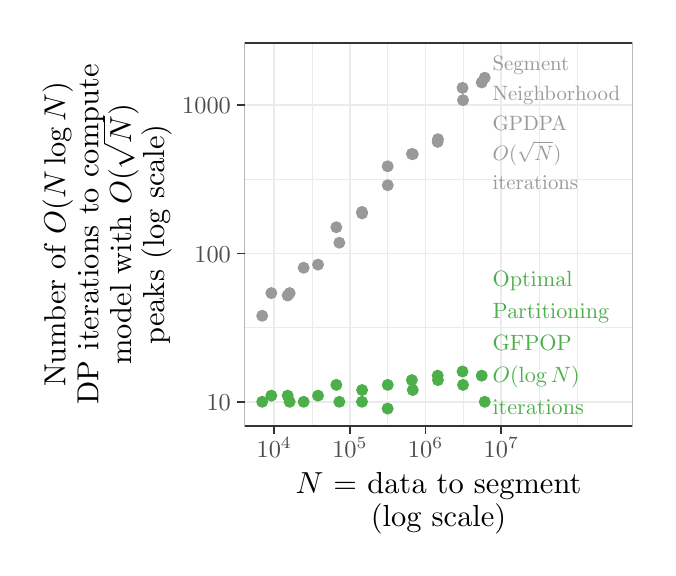
\begin{tikzpicture}[x=1pt,y=1pt]
\definecolor{fillColor}{RGB}{255,255,255}
\path[use as bounding box,fill=fillColor,fill opacity=0.00] (0,0) rectangle (224.04,187.90);
\begin{scope}
\path[clip] (  0.00,  0.00) rectangle (224.04,187.90);
\definecolor{drawColor}{RGB}{255,255,255}
\definecolor{fillColor}{RGB}{255,255,255}

\path[draw=drawColor,line width= 0.6pt,line join=round,line cap=round,fill=fillColor] (  0.00,  0.00) rectangle (224.04,187.90);
\end{scope}
\begin{scope}
\path[clip] ( 78.37, 43.96) rectangle (218.54,182.40);
\definecolor{fillColor}{RGB}{255,255,255}

\path[fill=fillColor] ( 78.37, 43.96) rectangle (218.54,182.40);
\definecolor{drawColor}{gray}{0.92}

\path[draw=drawColor,line width= 0.3pt,line join=round] ( 78.37, 79.52) --
	(218.54, 79.52);

\path[draw=drawColor,line width= 0.3pt,line join=round] ( 78.37,133.15) --
	(218.54,133.15);

\path[draw=drawColor,line width= 0.3pt,line join=round] (102.78, 43.96) --
	(102.78,182.40);

\path[draw=drawColor,line width= 0.3pt,line join=round] (130.13, 43.96) --
	(130.13,182.40);

\path[draw=drawColor,line width= 0.3pt,line join=round] (157.47, 43.96) --
	(157.47,182.40);

\path[draw=drawColor,line width= 0.3pt,line join=round] (184.82, 43.96) --
	(184.82,182.40);

\path[draw=drawColor,line width= 0.3pt,line join=round] (198.49, 43.96) --
	(198.49,182.40);

\path[draw=drawColor,line width= 0.6pt,line join=round] ( 78.37, 52.71) --
	(218.54, 52.71);

\path[draw=drawColor,line width= 0.6pt,line join=round] ( 78.37,106.34) --
	(218.54,106.34);

\path[draw=drawColor,line width= 0.6pt,line join=round] ( 78.37,159.97) --
	(218.54,159.97);

\path[draw=drawColor,line width= 0.6pt,line join=round] ( 89.11, 43.96) --
	( 89.11,182.40);

\path[draw=drawColor,line width= 0.6pt,line join=round] (116.45, 43.96) --
	(116.45,182.40);

\path[draw=drawColor,line width= 0.6pt,line join=round] (143.80, 43.96) --
	(143.80,182.40);

\path[draw=drawColor,line width= 0.6pt,line join=round] (171.15, 43.96) --
	(171.15,182.40);
\definecolor{drawColor}{gray}{0.60}
\definecolor{fillColor}{gray}{0.60}

\path[draw=drawColor,line width= 0.4pt,line join=round,line cap=round,fill=fillColor] ( 84.74, 83.80) circle (  1.96);

\path[draw=drawColor,line width= 0.4pt,line join=round,line cap=round,fill=fillColor] ( 88.04, 91.99) circle (  1.96);

\path[draw=drawColor,line width= 0.4pt,line join=round,line cap=round,fill=fillColor] ( 93.94, 91.11) circle (  1.96);

\path[draw=drawColor,line width= 0.4pt,line join=round,line cap=round,fill=fillColor] ( 94.67, 91.99) circle (  1.96);

\path[draw=drawColor,line width= 0.4pt,line join=round,line cap=round,fill=fillColor] ( 99.73,101.14) circle (  1.96);

\path[draw=drawColor,line width= 0.4pt,line join=round,line cap=round,fill=fillColor] (104.91,102.28) circle (  1.96);

\path[draw=drawColor,line width= 0.4pt,line join=round,line cap=round,fill=fillColor] (111.53,115.78) circle (  1.96);

\path[draw=drawColor,line width= 0.4pt,line join=round,line cap=round,fill=fillColor] (112.63,110.19) circle (  1.96);

\path[draw=drawColor,line width= 0.4pt,line join=round,line cap=round,fill=fillColor] (120.80,121.29) circle (  1.96);

\path[draw=drawColor,line width= 0.4pt,line join=round,line cap=round,fill=fillColor] (120.84,120.79) circle (  1.96);

\path[draw=drawColor,line width= 0.4pt,line join=round,line cap=round,fill=fillColor] (130.08,137.80) circle (  1.96);

\path[draw=drawColor,line width= 0.4pt,line join=round,line cap=round,fill=fillColor] (130.11,130.97) circle (  1.96);

\path[draw=drawColor,line width= 0.4pt,line join=round,line cap=round,fill=fillColor] (138.83,142.28) circle (  1.96);

\path[draw=drawColor,line width= 0.4pt,line join=round,line cap=round,fill=fillColor] (139.16,142.18) circle (  1.96);

\path[draw=drawColor,line width= 0.4pt,line join=round,line cap=round,fill=fillColor] (148.15,146.63) circle (  1.96);

\path[draw=drawColor,line width= 0.4pt,line join=round,line cap=round,fill=fillColor] (148.25,147.60) circle (  1.96);

\path[draw=drawColor,line width= 0.4pt,line join=round,line cap=round,fill=fillColor] (157.13,166.15) circle (  1.96);

\path[draw=drawColor,line width= 0.4pt,line join=round,line cap=round,fill=fillColor] (157.31,161.71) circle (  1.96);

\path[draw=drawColor,line width= 0.4pt,line join=round,line cap=round,fill=fillColor] (164.06,168.10) circle (  1.96);

\path[draw=drawColor,line width= 0.4pt,line join=round,line cap=round,fill=fillColor] (165.16,169.81) circle (  1.96);
\definecolor{drawColor}{RGB}{77,175,74}
\definecolor{fillColor}{RGB}{77,175,74}

\path[draw=drawColor,line width= 0.4pt,line join=round,line cap=round,fill=fillColor] ( 84.74, 52.71) circle (  1.96);

\path[draw=drawColor,line width= 0.4pt,line join=round,line cap=round,fill=fillColor] ( 88.04, 54.93) circle (  1.96);

\path[draw=drawColor,line width= 0.4pt,line join=round,line cap=round,fill=fillColor] ( 93.94, 54.93) circle (  1.96);

\path[draw=drawColor,line width= 0.4pt,line join=round,line cap=round,fill=fillColor] ( 94.67, 52.71) circle (  1.96);

\path[draw=drawColor,line width= 0.4pt,line join=round,line cap=round,fill=fillColor] ( 99.73, 52.71) circle (  1.96);

\path[draw=drawColor,line width= 0.4pt,line join=round,line cap=round,fill=fillColor] (104.91, 54.93) circle (  1.96);

\path[draw=drawColor,line width= 0.4pt,line join=round,line cap=round,fill=fillColor] (111.53, 58.82) circle (  1.96);

\path[draw=drawColor,line width= 0.4pt,line join=round,line cap=round,fill=fillColor] (112.63, 52.71) circle (  1.96);

\path[draw=drawColor,line width= 0.4pt,line join=round,line cap=round,fill=fillColor] (120.80, 52.71) circle (  1.96);

\path[draw=drawColor,line width= 0.4pt,line join=round,line cap=round,fill=fillColor] (120.84, 56.96) circle (  1.96);

\path[draw=drawColor,line width= 0.4pt,line join=round,line cap=round,fill=fillColor] (130.08, 50.26) circle (  1.96);

\path[draw=drawColor,line width= 0.4pt,line join=round,line cap=round,fill=fillColor] (130.11, 58.82) circle (  1.96);

\path[draw=drawColor,line width= 0.4pt,line join=round,line cap=round,fill=fillColor] (138.83, 60.55) circle (  1.96);

\path[draw=drawColor,line width= 0.4pt,line join=round,line cap=round,fill=fillColor] (139.16, 56.96) circle (  1.96);

\path[draw=drawColor,line width= 0.4pt,line join=round,line cap=round,fill=fillColor] (148.15, 62.15) circle (  1.96);

\path[draw=drawColor,line width= 0.4pt,line join=round,line cap=round,fill=fillColor] (148.25, 60.55) circle (  1.96);

\path[draw=drawColor,line width= 0.4pt,line join=round,line cap=round,fill=fillColor] (157.13, 63.66) circle (  1.96);

\path[draw=drawColor,line width= 0.4pt,line join=round,line cap=round,fill=fillColor] (157.31, 58.82) circle (  1.96);

\path[draw=drawColor,line width= 0.4pt,line join=round,line cap=round,fill=fillColor] (164.06, 62.15) circle (  1.96);

\path[draw=drawColor,line width= 0.4pt,line join=round,line cap=round,fill=fillColor] (165.16, 52.71) circle (  1.96);
\end{scope}
\begin{scope}
\path[clip] ( 78.37, 43.96) rectangle (218.54,182.40);
\definecolor{drawColor}{RGB}{77,175,74}

\node[text=drawColor,anchor=base west,inner sep=0pt, outer sep=0pt, scale=  0.80] at (168.00, 94.31) {Optimal};

\node[text=drawColor,anchor=base west,inner sep=0pt, outer sep=0pt, scale=  0.80] at (168.00, 82.79) {Partitioning};

\node[text=drawColor,anchor=base west,inner sep=0pt, outer sep=0pt, scale=  0.80] at (168.00, 71.27) {GFPOP};

\node[text=drawColor,anchor=base west,inner sep=0pt, outer sep=0pt, scale=  0.80] at (168.00, 59.75) {$O(\log N)$};

\node[text=drawColor,anchor=base west,inner sep=0pt, outer sep=0pt, scale=  0.80] at (168.00, 48.23) {iterations};
\definecolor{drawColor}{gray}{0.60}

\node[text=drawColor,anchor=base west,inner sep=0pt, outer sep=0pt, scale=  0.75] at (168.00,172.57) {Segment};

\node[text=drawColor,anchor=base west,inner sep=0pt, outer sep=0pt, scale=  0.75] at (168.00,161.74) {Neighborhood};

\node[text=drawColor,anchor=base west,inner sep=0pt, outer sep=0pt, scale=  0.75] at (168.00,150.91) {GPDPA};

\node[text=drawColor,anchor=base west,inner sep=0pt, outer sep=0pt, scale=  0.75] at (168.00,140.08) {$O(\sqrt N)$};

\node[text=drawColor,anchor=base west,inner sep=0pt, outer sep=0pt, scale=  0.75] at (168.00,129.25) {iterations};
\definecolor{drawColor}{gray}{0.20}

\path[draw=drawColor,line width= 0.6pt,line join=round,line cap=round] ( 78.37, 43.96) rectangle (218.54,182.40);
\end{scope}
\begin{scope}
\path[clip] (  0.00,  0.00) rectangle (224.04,187.90);
\definecolor{drawColor}{gray}{0.30}

\node[text=drawColor,anchor=base east,inner sep=0pt, outer sep=0pt, scale=  0.88] at ( 73.42, 49.46) {10};

\node[text=drawColor,anchor=base east,inner sep=0pt, outer sep=0pt, scale=  0.88] at ( 73.42,103.09) {100};

\node[text=drawColor,anchor=base east,inner sep=0pt, outer sep=0pt, scale=  0.88] at ( 73.42,156.71) {1000};
\end{scope}
\begin{scope}
\path[clip] (  0.00,  0.00) rectangle (224.04,187.90);
\definecolor{drawColor}{gray}{0.20}

\path[draw=drawColor,line width= 0.6pt,line join=round] ( 75.62, 52.71) --
	( 78.37, 52.71);

\path[draw=drawColor,line width= 0.6pt,line join=round] ( 75.62,106.34) --
	( 78.37,106.34);

\path[draw=drawColor,line width= 0.6pt,line join=round] ( 75.62,159.97) --
	( 78.37,159.97);
\end{scope}
\begin{scope}
\path[clip] (  0.00,  0.00) rectangle (224.04,187.90);
\definecolor{drawColor}{gray}{0.20}

\path[draw=drawColor,line width= 0.6pt,line join=round] ( 89.11, 41.21) --
	( 89.11, 43.96);

\path[draw=drawColor,line width= 0.6pt,line join=round] (116.45, 41.21) --
	(116.45, 43.96);

\path[draw=drawColor,line width= 0.6pt,line join=round] (143.80, 41.21) --
	(143.80, 43.96);

\path[draw=drawColor,line width= 0.6pt,line join=round] (171.15, 41.21) --
	(171.15, 43.96);
\end{scope}
\begin{scope}
\path[clip] (  0.00,  0.00) rectangle (224.04,187.90);
\definecolor{drawColor}{gray}{0.30}

\node[text=drawColor,anchor=base,inner sep=0pt, outer sep=0pt, scale=  0.88] at ( 89.11, 32.51) {$10^4$};

\node[text=drawColor,anchor=base,inner sep=0pt, outer sep=0pt, scale=  0.88] at (116.45, 32.51) {$10^5$};

\node[text=drawColor,anchor=base,inner sep=0pt, outer sep=0pt, scale=  0.88] at (143.80, 32.51) {$10^6$};

\node[text=drawColor,anchor=base,inner sep=0pt, outer sep=0pt, scale=  0.88] at (171.15, 32.51) {$10^7$};
\end{scope}
\begin{scope}
\path[clip] (  0.00,  0.00) rectangle (224.04,187.90);
\definecolor{drawColor}{RGB}{0,0,0}

\node[text=drawColor,anchor=base,inner sep=0pt, outer sep=0pt, scale=  1.10] at (148.45, 19.50) {$N$ = data to segment};

\node[text=drawColor,anchor=base,inner sep=0pt, outer sep=0pt, scale=  1.10] at (148.45,  7.62) {(log scale)};
\end{scope}
\begin{scope}
\path[clip] (  0.00,  0.00) rectangle (224.04,187.90);
\definecolor{drawColor}{RGB}{0,0,0}

\node[text=drawColor,rotate= 90.00,anchor=base,inner sep=0pt, outer sep=0pt, scale=  1.10] at ( 13.63,113.18) {Number of $O(N \log N)$};

\node[text=drawColor,rotate= 90.00,anchor=base,inner sep=0pt, outer sep=0pt, scale=  1.10] at ( 25.51,113.18) {DP iterations to compute};

\node[text=drawColor,rotate= 90.00,anchor=base,inner sep=0pt, outer sep=0pt, scale=  1.10] at ( 37.39,113.18) {model with $O(\sqrt N)$};

\node[text=drawColor,rotate= 90.00,anchor=base,inner sep=0pt, outer sep=0pt, scale=  1.10] at ( 49.27,113.18) {peaks (log scale)};
\end{scope}
\end{tikzpicture}
